
\subsection{Transformer Core Measurements}

As an alternate method of measuring changes in $\mu$, a method similar
to the standard method of magnetic materials characterization via
magnetic induction was used.  In this measurement technique, the
witness cylinder was used as the core of a transformer.  Two coils
(primary and secondary) were wound on the witness cylinder using
multistranded 20-gauge copper wire.  The windings were made as tight
as possible, but not so tight as to potentially stress the material.
The windings were not potted in place.

Each of the three witness cylinders was tested.  Data were acquired
using different numbers of turns on both the primary and secondary
coils (from six to 48 on the primary, and from 7 to 24 on the
secondary).
% Table 9 on page 65 of Taraneh's report shows the different windings.
% Can guess which core is which.

%In the end, a transformer with 48 windings on the primary and 21
%windings on the secondary was used.

%This enabled more saturation of the material.

The primary coil generated an AC magnetic field $H(t)$, while the
secondary coil was used to measure the EMF induced by the time-varying
magnetic flux and hence being proportional to $dB(t)/dt$.  To a good
approximation
\begin{equation}
H(t)=frac{N_pI(t)}{2\pi R}
\end{equation}
where $N_p$ is the number of turns in the primary, $I(t)$ is the
current in the primary, and $R$ is the radius of the witness cylinder,
and
\begin{equation}
\frac{dB(t)}{dt}=\frac{V(t)}{t\ell}
\end{equation}
where $V(t)$ is the voltage generated in the secondary, and $t$ and
$\ell$ are the thickness and length of the witness cylinder.

For a sinusoidal drive current $I(t)$, and under the assumption that
$B(t)=\mu H(t)$ with $\mu$ being a constant, the voltage generated in
the secondary $V(t)$ should be sinusoidal and out of phase with the
primary current.

The internal oscillator of a SRS830 lock-in amplifier was used to
generate $I(t)$.  This was monitored by measuring the voltage across a
1~$\Omega$ resistor with small temperature coefficient in the primary
loop.  The lock-in amplifier was then used to demodulate $V(t)$ into
its in-phase $X$ and out-of-phase $Y$ components.  The experiment was
done at 1 Hz and as small as possible $H(t)$, typically 0.1~A/m in
amplitude, to measure the slope of the minor $B-H$ loops near the
origin of the $B-H$ space.

The temperature of the core was measured at the same time as the sense
voltage using non-magnetic type T thermocouples.  Measurements of $Y$
as a function of temperature would then signify a change in $\mu$ with
temperature.  In general, we used ambient temperature variations, as
for our axial shielding factor measurements.

% Although we would have preferred to measure at even lower frequencies
% and amplitudes, these settings were found to be the minimum possible
% before noise would make it impossible to measurement the long-term
% (hours) evolution of the $X$ and $Y$ readings.

The naive expectation is that the out-of-phase $Y$ component should
signify a non-zero $\mu$, wherease the in-phase $X$ component should
be zero.  In practice, due to a combination of saturation, hysteresis,
eddy-current losses, and skin-depth effects, the $X$ component is
never zero.

It was found experimentally that the amplitude of $H(t)$ had to be
kept small compared to the coercivity ($\sim 3$~A/m) in order to
ensure that the $Y$ component was larger than the $X$ component.  This
is displayed graphically in Fig.~\ref{fig:data_and_simulation}, where
the dependence of $Y$ and $X$ on the amplitude of the applied $H(t)$
is displayed, for a driving frequency of 1~Hz are shown.  Clearly the
value of $X$ can be considerable compared to $Y$, for larger $H$
amplitudes near the coercivity.  At large amplitudes, the material
goes into saturation, and both $Y$ and $X$ eventually decrease at
amplitudes much greater than the coercivity.  This behavior, and
signal-to-noise considerations, drove our decision to measure at
typically 0.1~A/m amplitude and 1~Hz.

The observation of nonzero $X$ signal is due to effects such as
hysteresis, saturation, eddy currents, and skin depth.  Therefore, it
is not truly possible to embody the results as a single parameter
$\mu$, although we desired to express our results as such.  To
understand the behavior in Fig.~\ref{fig:data_and_simulation} effects,
a theoretical model of the hysteresis based on Jiles~\cite{bib:jiles}
was used.

The key parameters of Jiles' model are saturation magnetization $M_s$,
mean field parameter $\alpha$ which represents interdomain coupling,
$a$ with the dimensions of magnetic field which characterizes the
shape of anhysteretic magnetization, bulk magnetization $M$ and the
magnetic field $H$.  We adjusted these parameters based on our
separate measurements of $B-H$ loops including the initial
magnetization curve.  These measurements were done at frequencies from
0.01 to 10~Hz.  It was found that the frequency dependence predicted
by Ref.~\cite{bib:jiles} gave relatively good agreement with the
measured B-H loops once the five original
(Jiles-Atherton~\cite{bib:ja}) parameters were tuned.  These same
parameters were then used to model the measurement presented in
Fig.~\ref{fig:data_and_simulation}, including the lock-in amplifier
function.  As shown in Fig.~\ref{fig:data_and_simulation}, trends in
the measurements and simulations are fairly consistent.  The sign of
$X$ relative to $Y$ is also correctly predicted by the model (we have
adjusted them both to be positive, for graphing purposes).  We think
that with further tuning of the model, even better agreement could be
gotten.

\begin{figure}[h!]
\begin{center}
   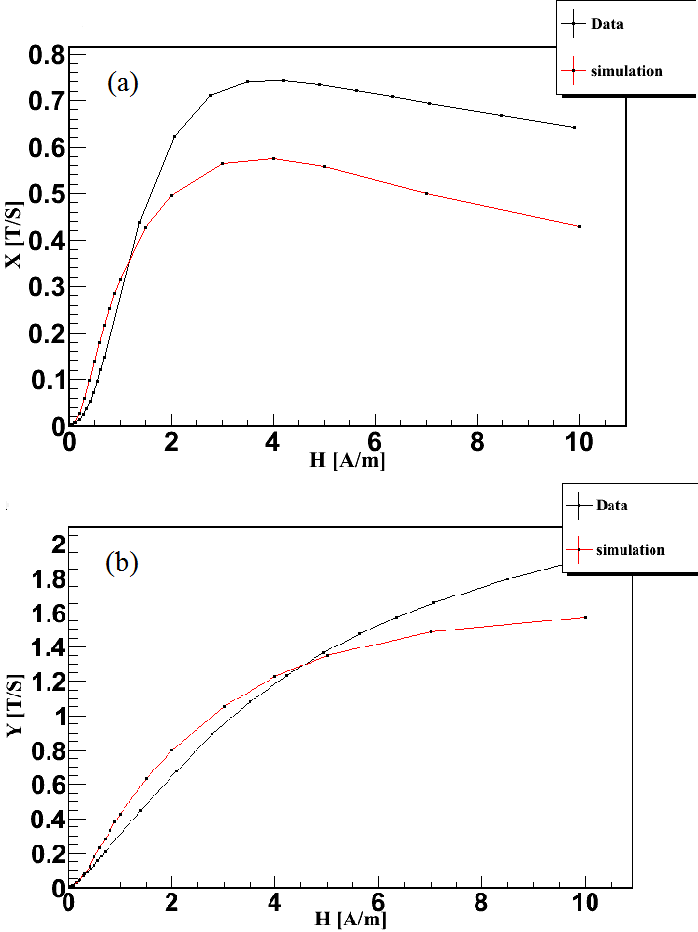
\includegraphics[width=0.5\textwidth]{data_and_simulation3.PNG}
    \caption{These graphs represent the sense voltage as a function of applied $H$ field at 1~Hz. Graph (a) shows the out-of-phase component $X$ of the measured sense voltage as well as the simulation. Graph (b) shows the in-phase component $Y$ of the signal and its simulation.}
    \label{fig:data_and_simulation}
    \end{center}
% Jeff to do: fix figure caption once this section (and this figure)
% are complete.
\end{figure} 


The $Y$ and $X$ signals are therefore reminiscent of a complicated set
of parameters embodying hysteresis and other losses in the sample.
This draws into question the practice of using $Y(T)$ as an indication
of the temperature dependence of the magnetic permeability $\mu(T)$.

We nonetheless took data on $Y(T)$ which we naively interpret as
$\mu(T)$.  We assign no additional systematic error for this
simplification, and all our results are subject to this caveat.  We
comment further that in our measurements of the axial shielding
factor, the same caveat exists.  In that case one would expect the
in-phase $X$ component to dominate the demodulated fluxgate signal.
While it does dominate, the $Y$ component is never exactly zero.  In a
sense, measuring $\mu(T)$ itself is always an approximation, since it
is actually the parameters of minor loops in a hysteresis curve which
are measured.  Our results may be interpreted as a measure of the
temperature-dependence of the slopes of those minor loops.

Graphs of $\frac{1}{Y}\frac{dY}{dT}$ as a function of $T$ were made.
In general, the data mimicked the behavior of the axial shielding
factor measurements, giving a similar level of linearity with
temperature as the data displayed in
Fig.~\ref{fig:figure_from_axial_tex}.  Other similar behaviors to
those measurement were also observed, for example: (a) when the
temperature slope changed sign, $Y$ would temporarily give a different
slope with temperature, (b) the overall slope of $1/Y dY/dT$ depended
on a variety of factors, most notably a dependence on which of the
three witness cylinders was used for the measurement, and on
differences between subsequent measurements using the same cylinder.

Based on a number of measurements with different cores and windings,
the data showed a range of 0.1\%/K to 2.1\%/K for
$\frac{1}{\mu}\frac{d\mu}{dT}=\frac{1}{Y}\frac{dY}{dT}$, again naively
assuming the material to be linear as discussed above.  The sign of
the slope with temperature was the same as the axial shielding factor
technique.

We discuss further systematic errors affecting the measurement in the
next section.

\subsubsection{Systematic Errors}

% 1.  Focus on unique ones:
% - motion of wires (done)
% - degaussing, how done, and general observations (done)
% - resistance of wires (done)
% - different numbers of turns on primary/secondary  (Taraneh: talked about it earlier)
% - in-phase/out-of-phase components, how small should in-phase be? (Taraneh: talked about it already.)
% - background noise (done)
% - ...

% 2.  Or if there are any other ones that are from the same source
% (e.g. resistance of wire might be in this category) but the value is
% different for some reason

% 3.  Or if some are eliminated, it would be good to note here, for
% example, fluxgate systematics and some classes of motion systematics
% (done-> just for fluxgate)


The dominant source of variation between results in this method arose
from properties inherent to each witness cylinder.  One of the
cylinders gave temperature slopes consistently larger
$\frac{1}{Y}\frac{dY}{dT}\sim 1.2-2.1$\%/K than the other two
$\frac{1}{Y}\frac{dY}{dT}\sim 0.1-0.7$\%/K.  We expect this indicates
some difference in the annealing process or subsequent treatment of
this cylinder, although to our knowledge the treatment was controlled
the same as for the other two cylinders.

Since our goal is to provide input to future EDM experiments on the
likely scale of the temperature dependence of $\mu$ that they can
expect, we phrase our result as a range covering all these results.
% However, it is possible that through improved control of the annealing
% process or of the treatment of the material, the smaller of these two
% slopes could be selected.

In this method the secondary voltage $V(t)$ was measured directly by a
lock-in amplifier and so systematics correlated to fluxgate were
removed, compared with the axial shielding factor measurement.  This
method therefore addresses possible systematic drifts in fluxgate
performance.  It is clear that these were unlikely to dominate the
errors in the axial shielding factor measurements.


A possible systematic effect arises due to settling or slight motions
of the wires used to wind the primary and secondary coils on the
witness cylinders.  The coils were wound by hand directly onto the
witness cylinder and were held in place by tension.
%The systematic
%effect on the induced EMF in the secondary is expected to be small,
%because the flux through a coil that is deformed would be the same as
%as that of a perfect coil.  The situation is less clear for the
%primary coil, but we also anticipate this effect to be small, because
%we expect magnetic field lines to be strongly contained by the core.
%Furthermore, i
In shorter time measurements when the temperature was not changing,
the $Y$ and $X$ values generally did not change at the $<0.1\%$ level.
We do not assign any additional systematic error for possible motion
of the windings.

%degaussing
Detailed measurements of the effect of degaussing were conducted for
this geometry.  In fact, the ability to degauss led us ultimately to
select a larger number of primary turns (48) so that we could fully
saturate the core using only the lock-in amplifier reference output as
a current source.

A computer program was used to control the lock-in amplifier in order
to implement degaussing.  A sine wave with the measurement frequency
(typically 1~Hz) was applied at the maximum lock-in output power.
Over the course of several thousand oscillations, the amplitude was
decreased linearly to the measurement amplitude ($\sim 0.1$~A/m).  A
possible limitation of this system is that the lock-in amplifier could
only be programmed to change its amplitude at the level of 12 bits of
precision; we did not study the effect of this in further detail.

An immediately obvious effect was that the $Y$ and $X$ values after
degaussing were normally larger than prior to degaussing.  We
interpret this difference as an increase in the effective $\mu$.

The temperature dependence of $Y$ (and effective $\mu$) did not change
significantly.  Poor degaussing (for example, degaussing with too few
cycles, or ramping too rapidly to zero) could result significantly
different initial slopes with temperature, where the effective $\mu$
would drift for several hours after degaussing.  But after improving
the system to have a large number of cycles (consistent with the
recommendations of Refs.~\cite{bib:thiel}) the results became
consistent with being affected by temperature changes, and were also
consistent with previous measurements were no degaussing was done.

To check the stability of the applied current in the primary coil,
voltage across a 1~$\Omega$ temperature controlled resistor in series
with the primary coil was demodulated using a second lock-in
amplifier.  The result showed $<0.1$\%/K changes in current ruling out
this as an additional source of systematic error.

To reduce the background noise and thermally isolate the witness
cylinder, most measurements were done by placing the witness cylinder
inside the prototype passive shield.  The results did not show a
significant change whether they were done with the caps of the
prototype passive shield on or off.  The results were even consistent
when done outside the passive shields.


%\begin{itemize}
%\item Describe experimental setup and important consdierations (e.g. relationship of data to effective $%\mu$)
%\item Explain B, H, f, and dominant systematic effects.
%\item Understanding in terms of Jiles-Atherton.  Complications that
 % this does not translate well into ``$\mu$''.
%\item One data graph?  (Perhaps the Jiles-Atherton one?)
%\item State overall result and systematic error.
%\end{itemize}


To summarize, the dominant systematic effects arose due to different
similarly prepared cores giving different results, and due to
variations in the measured slopes in multiple measurements on the same
core.  The second of these is essentially the same error encountered
in our axial shielding factor measurements.  We expect it has the same
source; it is likely due to some property of the material the cores
are made of, or an additional unknown systematic uncertainty.

Finally we note the primary caveat to these measurements, discussed
above, which is that both measurements (transformer core and axial
shielding factor) do not truly measure $\mu$.  Rather they measure
observables related to the slope of minor hysteresis loops in B-H
space.  They would be more appropriately described by a model like
that of Jiles~\cite{bib:jiles}, but to extract the temperature
dependence of the five parameters of the model is beyond the scope of
this work.  Instead we acknowledge this fact and relate the
temperature dependence of the effective $\mu$ measured by each
experiment.

We think it is interesting and useful information that the two
experiments measure the same scale and sign of the temperature
dependence of their respective effective $\mu$'s.  We feel this is the
principal contribution of this work.
